\documentclass[a4paper, 12pt]{article}		% general format
\usepackage{multicol}
%%%% Charset
\usepackage{cmap}							% make PDF files searchable and copyable
\usepackage[utf8x]{inputenc} 				% accept different input encodings
\usepackage[english,russian]{babel}   %% загружает пакет многоязыковой вёрстки
\usepackage{fontspec}      %% подготавливает загрузку шрифтов Open Type, True Type и др.
\defaultfontfeatures{Ligatures={TeX},Renderer=Basic}  %% свойства шрифтов по умолчанию
\setmainfont[Ligatures={TeX,Historic}]{Roboto-Light} %% задаёт основной шрифт документа
\setsansfont{Roboto-Light}  
\usepackage{float}
%%%% Graphics
\usepackage[dvipsnames]{xcolor}			% driver-independent color extensions
\usepackage{graphicx}						% enhanced support for graphics
\usepackage{wrapfig}						% produces figures which text can flow around
\usepackage{hyperref}
%%%% Math
\usepackage{amsmath}						% American Mathematical Society (AMS) math facilities
\usepackage{amsfonts}						% fonts from the AMS
\usepackage{amssymb}						% additional math symbols

%%%% Typograpy (don't forget about cm-super)
\usepackage{microtype}						% subliminal refinements towards typographical perfection
\linespread{1.3}							% line spacing
\usepackage[left=2.5cm, right=1.5cm, top=2.5cm, bottom=2.5cm]{geometry}
\setlength{\parindent}{0pt}					% we don't want any paragraph indentation
\usepackage{parskip}						% some distance between paragraphs

%%%% Tables
\usepackage{tabularx}						% tables with variable width columns
\usepackage{multirow}						% for tabularx
\usepackage{hhline}							% for tabularx
\usepackage{tabu}
\usepackage{longtable}

%%%% Graph
\usepackage{tikz}							% package for creating graphics programmatically
\usetikzlibrary{arrows}						% edges for tikz

%%%% Other
\usepackage{url}							% verbatim with URL-sensitive line breaks
\usepackage{fancyvrb}						% sophisticated verbatim text (with box)

\usepackage{listings}
\usepackage{caption}
\DeclareCaptionFont{white}{\color{white}}
\DeclareCaptionFormat{listing}{\colorbox{gray}{\parbox{\dimexpr\textwidth-1.72\fboxsep\relax}{#1#2#3}}}
\captionsetup[lstlisting]{format=listing,labelfont=white,textfont=white,margin=0pt}
\lstset{language=C,
	basicstyle=\footnotesize,
	keepspaces=true,
	tabsize=4,               
	frame=single,                           % Single frame around code
	rulecolor=\color{black},
	captionpos=b,
	showstringspaces=false,	
	abovecaptionskip=-0.9pt,
	xleftmargin=3.4pt,
	xrightmargin=2.6pt,
	breaklines=true,
	postbreak=\raisebox{0ex}[0ex][0ex]{\ensuremath{\color{black}\hookrightarrow\space}},
	xleftmargin=3.2pt,
	literate={а}{{\selectfont\char224}}1
	{~}{{\textasciitilde}}1
	{б}{{\selectfont\char225}}1
	{в}{{\selectfont\char226}}1
	{г}{{\selectfont\char227}}1
	{д}{{\selectfont\char228}}1
	{е}{{\selectfont\char229}}1
	{ё}{{\"e}}1
	{ж}{{\selectfont\char230}}1
	{з}{{\selectfont\char231}}1
	{и}{{\selectfont\char232}}1
	{й}{{\selectfont\char233}}1
	{к}{{\selectfont\char234}}1
	{л}{{\selectfont\char235}}1
	{м}{{\selectfont\char236}}1
	{н}{{\selectfont\char237}}1
	{о}{{\selectfont\char238}}1
	{п}{{\selectfont\char239}}1
	{р}{{\selectfont\char240}}1
	{с}{{\selectfont\char241}}1
	{т}{{\selectfont\char242}}1
	{у}{{\selectfont\char243}}1
	{ф}{{\selectfont\char244}}1
	{х}{{\selectfont\char245}}1
	{ц}{{\selectfont\char246}}1
	{ч}{{\selectfont\char247}}1
	{ш}{{\selectfont\char248}}1
	{щ}{{\selectfont\char249}}1
	{ъ}{{\selectfont\char250}}1
	{ы}{{\selectfont\char251}}1
	{ь}{{\selectfont\char252}}1
	{э}{{\selectfont\char253}}1
	{ю}{{\selectfont\char254}}1
	{я}{{\selectfont\char255}}1
	{А}{{\selectfont\char192}}1
	{Б}{{\selectfont\char193}}1
	{В}{{\selectfont\char194}}1
	{Г}{{\selectfont\char195}}1
	{Д}{{\selectfont\char196}}1
	{Е}{{\selectfont\char197}}1
	{Ё}{{\"E}}1
	{Ж}{{\selectfont\char198}}1
	{З}{{\selectfont\char199}}1
	{И}{{\selectfont\char200}}1
	{Й}{{\selectfont\char201}}1
	{К}{{\selectfont\char202}}1
	{Л}{{\selectfont\char203}}1
	{М}{{\selectfont\char204}}1
	{Н}{{\selectfont\char205}}1
	{О}{{\selectfont\char206}}1
	{П}{{\selectfont\char207}}1
	{Р}{{\selectfont\char208}}1
	{С}{{\selectfont\char209}}1
	{Т}{{\selectfont\char210}}1
	{У}{{\selectfont\char211}}1
	{Ф}{{\selectfont\char212}}1
	{Х}{{\selectfont\char213}}1
	{Ц}{{\selectfont\char214}}1
	{Ч}{{\selectfont\char215}}1
	{Ш}{{\selectfont\char216}}1
	{Щ}{{\selectfont\char217}}1
	{Ъ}{{\selectfont\char218}}1
	{Ы}{{\selectfont\char219}}1
	{Ь}{{\selectfont\char220}}1
	{Э}{{\selectfont\char221}}1
	{Ю}{{\selectfont\char222}}1
	{Я}{{\selectfont\char223}}1,
	extendedchars=true
}

%галочка
\usepackage{amssymb}% http://ctan.org/pkg/amssymb
\usepackage{pifont}% http://ctan.org/pkg/pifont
\newcommand{\cmark}{\ding{52}}%
\newcommand{\xmark}{\ding{56}}
%------------------------------------------------------------------------------
\renewcommand{\labelenumii}{\theenumii}
\renewcommand{\theenumii}{\theenumi.\arabic{enumii}.}
\begin{document}
%------------------------------------------------
	\begin{titlepage}
		\begin{center}
			\large {Санкт-Петербургский политехнический университет Петра Великого\\
				Институт компьютерных наук и технологий}\\
		\end{center}
		\begin{center}
			\large\textbf {Кафедра компьютерных систем и программных технологий}
		\end{center}
		\vfill
		\begin{center}
			\large{\textbf{Отчет о лабораторной работе №5} \\
			\textbf{Курс: } Администрирование компьютерных сетей\\
			\textbf{Тема: } Перенос сети в Cisco Packet Tracer}
		\end{center}
		
		\vfill
		
		\flushleft{Выполнил студент группы 13541/3} 
		\hfill\parbox{9 cm}{\hspace*{3cm}\hbox to 0cm{\raisebox{-1em}{\small(подпись)}}\hspace*{-0.8cm}\rule{3cm}{0.8pt} Д.В. Круминьш}\\[0.6cm]
		
		\flushleft{Преподаватель} \hfill\parbox{9 cm}{\hspace*{3cm}\hbox to 0cm{\raisebox{-1em}{\small(подпись)}}\hspace*{-0.8cm}\rule{3cm}{0.8pt} И.А. Малышев}\\[0.6cm]
		
		\vspace{\fill}
		\begin{center}
			Санкт-Петербург \\ 2018 г.
		\end{center}
	\end{titlepage}
%------------------------------------------------
\setcounter{page}{2}
%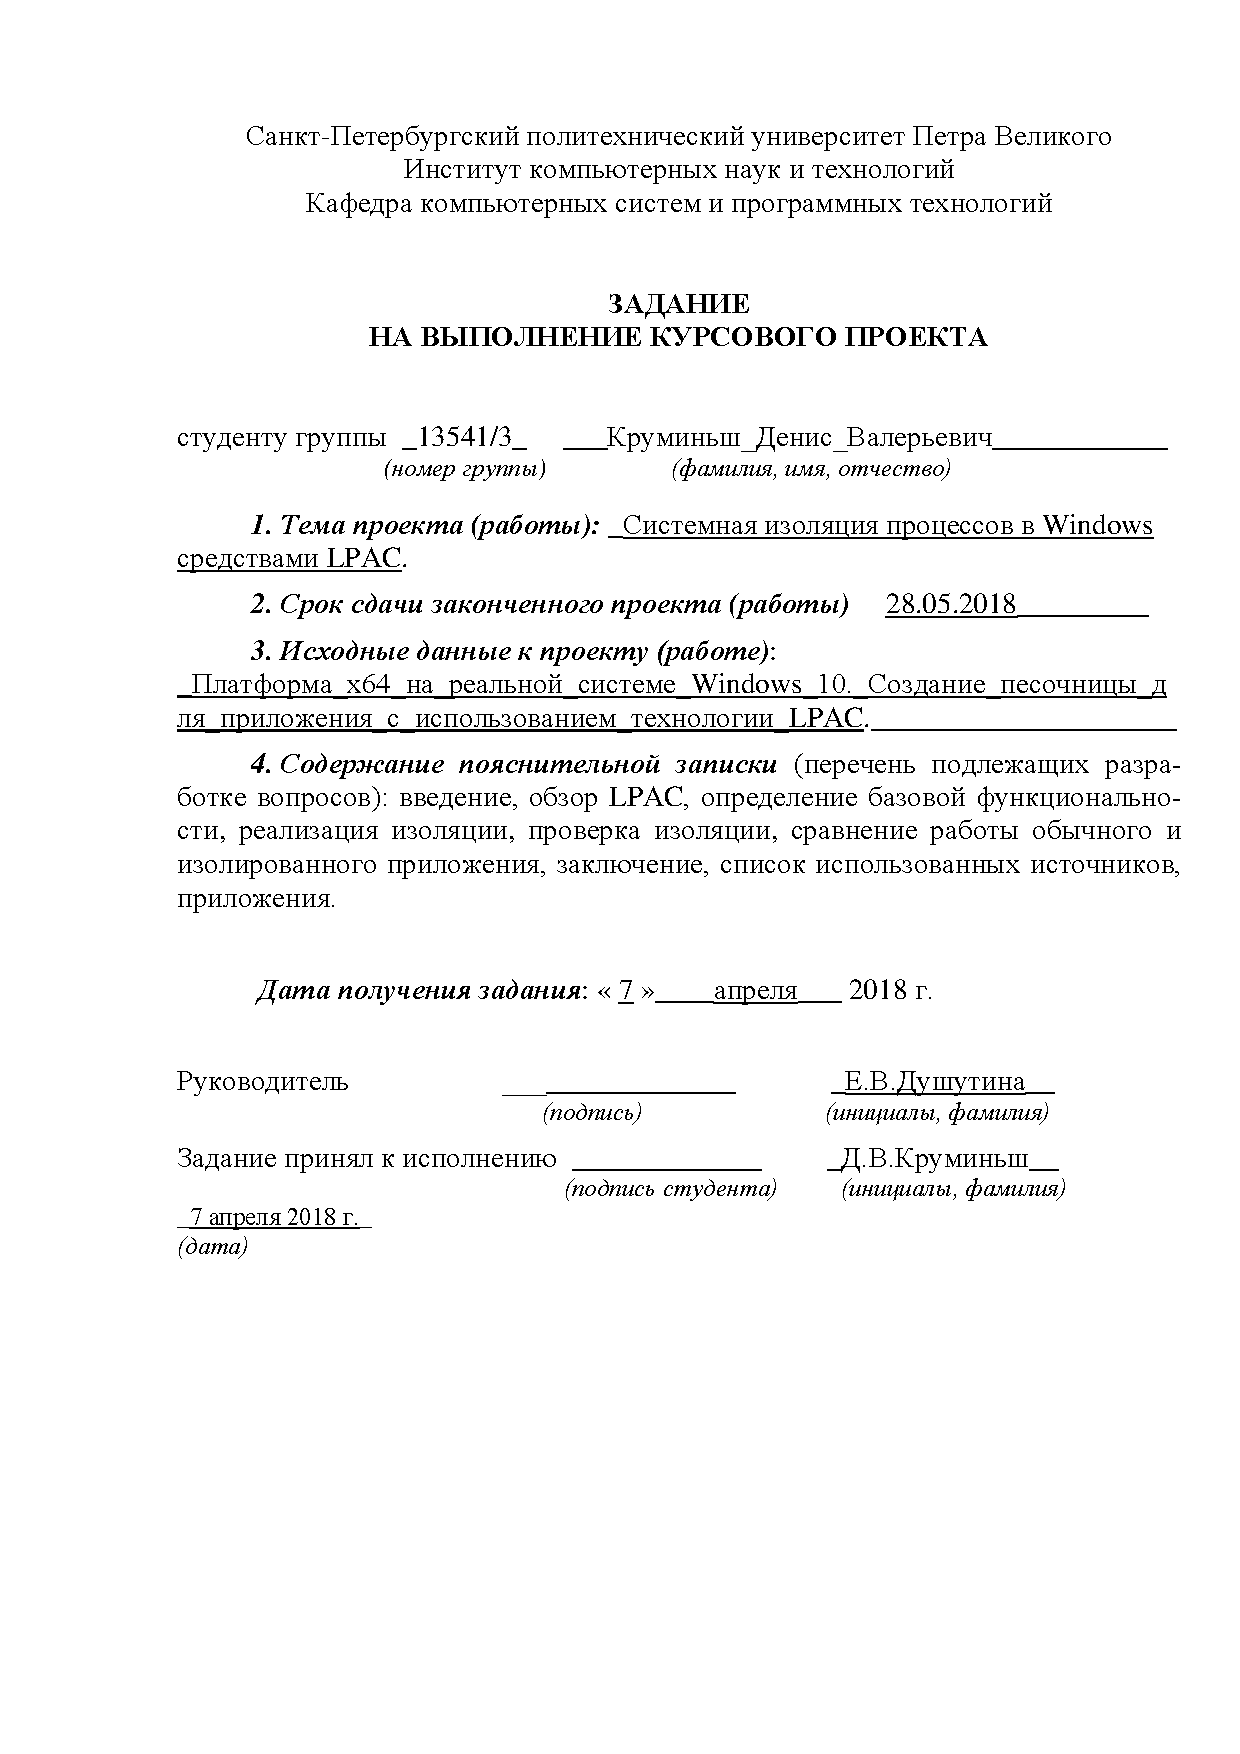
\includepdf[pages=-,pagecommand={},width=\textwidth]{task.pdf}
\tableofcontents
\clearpage

%------------------------------------------------------------------------------
%\input{intro}

\addcontentsline{toc}{section}{Введение}
\section*{Введение}
Современные серверы обладают избыточной производительностью, и приложения порой не используют даже их части. В результате системы какое-то время «простаивают», вместо выполнения полезной работы. Выходом стала виртуализация, позволяющая запускать несколько ОС на одном сервере, гарантированно разделяя их между собой и выделяя каждой нужное количество ресурсов. Но прогресс не стоит на месте. Следующий этап — \textbf{микросервисы}, когда каждая часть приложения развертывается отдельно, как самодостаточный компонент, который легко масштабируется под нужную нагрузку и обновляется. 

Изоляция предотвращает вмешательство в работу микросервиса со стороны других приложений. С появлением проекта Docker, упростившего процесс упаковки и доставки приложений вместе с окружением, архитектура микросервисов получила дополнительный толчок в развитии.

Проект Docker нативен для Linux систем, но для систем семейства Windows, приходилось ставить виртуальную машину, что является достаточно громоздким решением.

И совсем недавно, в ОС семейства Windows появились свои, нативные контейнеры - \textbf{Application Container} и \textbf{LPAC} - Less Privileged Application Container.
\clearpage

\section{Обзор LPAC}
Контейнеры — это способ разместить приложение в собственной изолированной «коробке». У приложения в контейнере нет сведений о других приложениях или процессах, размещенных за пределами этой «коробки». Все необходимое приложению для успешной работы также находится в этом контейнере. Куда бы контейнер не переместить, приложение всегда будет работать, так как оно получит все необходимое для запуска.

Контейнеры появились сравнительно недавно, где LPAC является частным случаем Application Container:
\begin{itemize}
\item \textbf{AC} - Application Container
\begin{itemize}
\item Появился в Windows Server 2016;
\item Разработчики были вдохновлены успехами Docker(Linux).
\end{itemize}
\item \textbf{LPAC} - Less Privileged Application Container
\begin{itemize}
\item Появился в Windows 10 Creators Update(2017 год).
\end{itemize}
\end{itemize}

Причины использования контейнеров:
\begin{itemize}
\item Легкая переносимость приложений;
\begin{itemize}
\item Так как контейнер содержит все необходимое для запуска приложения, он отличается высокой переносимостью и может запускаться на любом компьютере под управлением Windows Server 2016 и ОС старше.
\end{itemize}
\item Востребованность при использовании микросервисов.
\end{itemize}



\subsection{Принципы работы контейнера}
Контейнеры — это изолированная и переносимая среда выполнения с контролируемыми ресурсами, которая работает на хост-компьютере или виртуальной машине. Приложения или процессы, которые запускаются в контейнере, поставляются вместе со всеми необходимыми компонентами и файлами конфигурации. Они не имеют представления о других процессах, выполняющихся вне контейнера.

Узел контейнера предоставляет набор ресурсов, и контейнер будет использовать только их. Контейнер считает, что других ресурсов, помимо предоставленных, не существует, поэтому он не может взаимодействовать с ресурсами, выделенными соседнему контейнеру.

При создании контейнеров Windows и последующей работе с ними пригодятся перечисленные ниже основные понятия.

\textbf{Узел контейнера.} Физический или виртуальный компьютер, настроенный для работы с контейнерами Windows. На узле контейнера работает один или несколько контейнеров Windows.


\textbf{Образ контейнера.} По мере того как в файловую систему или реестр контейнера вносятся изменения (например, при установке программного обеспечения), они регистрируются в "песочнице". Во многих случаях может потребоваться зарегистрировать это состояние, чтобы применить внесенные изменения при создании новых контейнеров. В этом и заключается суть образа:после остановки работы контейнера можно либо отключить "песочницу", либо преобразовать ее в новый образ контейнера. Предположим, что в контейнер происходит установка MySQL. Создание нового образа на базе этого контейнера будет происходить аналогично его развертыванию. Этот образ будет содержать только внесенные изменения (MySQL) и при этом работать в виде слоя поверх образа ОС контейнера.

\textbf{"Песочница".} После запуска контейнера все операции записи (изменения файловой системы и реестра либо установка программного обеспечения) регистрируются на уровне "песочницы".

\textbf{Образ ОС контейнера.} Контейнеры развертываются из образов. Образ ОС контейнера— это первый из возможного множества слоев образа, составляющих контейнер. Этот образ представляет собой среду операционной системы. Образ ОС контейнера невозможно изменить.

\textbf{Репозиторий контейнера.} При каждом создании образа контейнера этот образ и его зависимости сохраняются в локальном репозитории. Эти образы можно использовать повторно много раз на узле контейнера. Образы контейнеров также можно хранить в открытом или закрытом реестре (например, Docker Hub), чтобы использовать на многих других узлах контейнеров.

\begin{figure}[H]
  \centering
  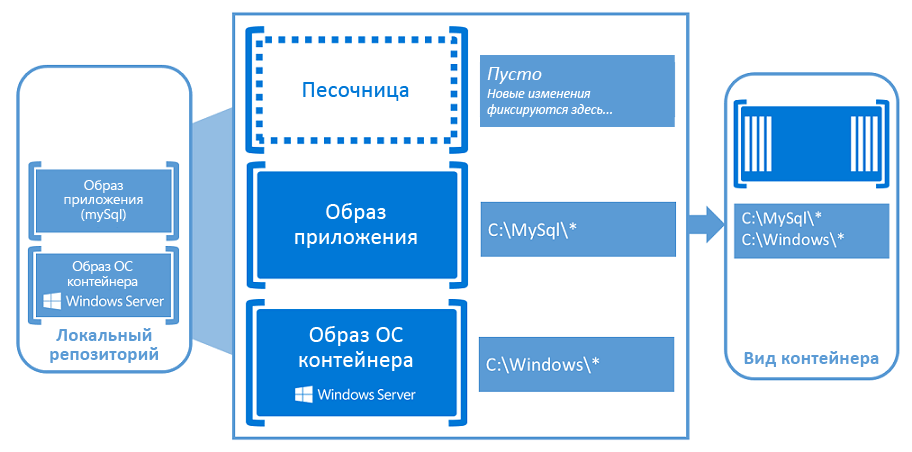
\includegraphics[width=\textwidth]{img/containerfund}
  \caption{Взаимодействие с контейнерами}
\end{figure}
Отличие контейнеров от виртуальных машин заключается в том, что контейнеры не загружают собственные копии ОС, библиотеки, системные файлы и прочее.перационная система как бы делится с контейнером. Единственное, что дополнительно требуется, — это ресурсы, необходимые для запуска приложения в контейнере. В результате контейнер стартует в считаные секунды и меньше нагружает систему, чем в случае применения виртуальных машин.

Подобно \textbf{Docker} имеются тенденции к развитию репозиториев с контейнерами, то есть к распространению уже предварительно настроенных контейнеров, с опреленными функциями.

Контейнеры Windows используют одно ядро с ОС, которое динамично разделяют между собой. Процесс распределения (CPU, ОЗУ, сеть) берет на себя ОС. При необходимости можно ограничить максимально доступные ресурсы, выделяемые контейнеру. Файлы ОС и запущенные службы проецируются в пространство имен каждого контейнера. Такой тип контейнера эффективно использует ресурсы, уменьшая накладные расходы, а значит, позволяет более плотно размещать приложения.\\\\
\textbf{Микросервисы}\\
Наиболее прибыльной и востребованной тенденцией для использования контейнеров являются микросервисы. Микросервис - это подход к разработке приложений, где каждая часть приложения развертывается как полностью автономный компонент, называемый микросервисом, который можно индивидуально масштабировать и обновлять. Например, подсистема приложения, которая получает запросы из общедоступного Интернета, может быть отделена от подсистемы, которая помещает запрос в очередь для поддержки бэкэнд-подсистемы и перебрасывает их в базу данных.

Микросервис - это не новый подход, и он явно не привязан к контейнерам, но преимущества контейнеров увеличиваются при применении к сложному приложению на основе микросервиса. Это означает, что микросервис может быстро масштабироваться, чтобы удовлетворить повышенную нагрузку, пространство имен и изоляция ресурсов контейнеров не позволяет одному экземпляру микросервиса вмешиваться в другие.

\subsection{Оркестраторы контейнера}
Благодаря малому размеру и ориентированности на приложение контейнеры удобно применять в средах с гибкой настройкой доставки и архитектурах, основанных на микрослужбах. Однако, при использовании контейнеров и микрослужб можно внедрить в свою среду сотни и тысячи компонентов. Можно вручную управлять несколькими десятками виртуальных машин и физических серверов, но не существует способа управления средой контейнеров промышленного масштаба без средств автоматизации. Автоматизация большого количества контейнеров и управление ими, а также их взаимодействиями называется оркестрацией.

Стандартное определение оркестрации включает следующие задачи:
\begin{itemize}
\item \textbf{Планирование}: поиск подходящего компьютера для запуска контейнера с учетом образа контейнера и запроса на ресурс. Сходство или удаление сходства: указать, что контейнеры в наборе должны запускаться рядом друг с другом (для повышения производительности) или достаточно далеко друг от друга (для обеспечения доступности).
\item \textbf{Наблюдение за работоспособностью}: отслеживание сбоев контейнера и автоматическое изменение расписания для него.
\item \textbf{Отработка отказа}: отслеживание запущенных задач на каждой машине и переназначение контейнеров с машин, на которых возник сбой, на работоспособные узлы.
\item \textbf{Масштабирование}: добавление или удаление экземпляров контейнера для соответствия запросу (ручное или автоматическое).
\item \textbf{Сеть}: предоставление сети наложения для координации контейнеров при обмене данными между несколькими хост-машинами.
\item \textbf{Обнаружение служб}: обеспечение автоматической локализации контейнеров даже при перемещении между хост-машинами и изменении IP-адреса.
\item \textbf{Координация обновления приложений}: управление обновлениями контейнера во избежание простоев и откат до предыдущей версии в случае сбоя.
\end{itemize}



\subsection{Аналоги}
\subsubsection{FreeBSD Jail}
Jails основывается на концепции chroot (2), которая используется для изменения корневого каталога набора процессов. Это создает безопасную среду, отдельную от остальной части системы. Процессы, созданные в среде chrooted, не могут получить доступ к файлам или ресурсам за ее пределами. По этой причине компрометация службы, запущенной в chrooted-среде, не должна позволять злоумышленнику изменять внутренности системы. Однако, chroot имеет несколько ограничений. Он подходит для простых задач, которые не требуют большой гибкости или сложных, расширенных функций. Со временем было обнаружено, что многие способы избавиться от chrooted среды, что делает его менее идеальным решением для обеспечения безопасности.

Jails улучшают концепцию традиционной среды chroot несколькими способами. В традиционной среде chroot процессы ограничены только в той части файловой системы, к которой они могут получить доступ. Остальные системные ресурсы, системные пользователи, запущенные процессы и сетевая подсистема совместно используются chrooted процессами и процессами хост-системы. Jails расширяет эту модель путем виртуализации доступа к файловой системе, набору пользователей и сетевой подсистеме. Доступны более мелкозернистые элементы управления для настройки доступа к Jails. Jails можно рассматривать как тип виртуализации на уровне операционной системы.


Находясь "за решеткой", root не имеет прав:
\begin{itemize}
\item Загружать модули ядра и каким-либо образом модифицировать ядро (например, через /dev/kmem).
\item Изменять переменные ядра (за исключением kern.securelevel и kern.hostname).
\item Создавать файлы устройств.
\item Монтировать и демонтировать файловые системы.
\item Изменять сетевые конфигурации.
\item Создавать raw сокеты (поведение настраивается).
\item Получать доступ к сетевым ресурсам, не ассоциированным с IP-адресом jail’а.
\item Работать с System V IPC (поведение настраивается).
\item Присоединяться к процессу и использовать ptrace(2).
\end{itemize}

\subsubsection{Docker}
Docker - одна из самых популярных платформ для работы с контейнерами для Linux.

В своем ядре docker позволяет запускать практически любое приложение, безопасно изолированное в контейнере. Безопасная изоляция позволяет вам запускать на одном хосте много контейнеров одновременно. Легковесная природа контейнера, который запускается без дополнительной нагрузки гипервизора, позволяет вам добиваться больше от вашего железа.

Основа изоляции лежит на пространстве имен и контрольных группах.

\textbf{Пространство имен(namespaces)}\\
Docker использует технологию namespaces для организации изолированных рабочих пространств, которые мы называем контейнерами. Когда мы запускаем контейнер, docker создает набор пространств имен для данного контейнера.

Это создает изолированный уровень, каждый аспект контейнера запущен в своем простанстве имен, и не имеет доступ к внешней системе.

Список некоторых пространств имен, которые использует docker:
\begin{itemize}
\item pid: для изоляции процесса;
\item net: для управления сетевыми интерфейсами;
\item ipc: для управления IPC ресурсами. (ICP: InterProccess Communication);
\item mnt: для управления точками монтирования;
\item utc: для изолирования ядра и контроля генерации версий(UTC: Unix timesharing system).
\end{itemize}
\textbf{Control groups (контрольные группы)}\\
Docker также использует технологию cgroups или контрольные группы. Ключ к работе приложения в изоляции, предоставление приложению только тех ресурсов, которые вы хотите предоставить. Это гарантирует, что контейнеры будут хорошими соседями. Контрольные группы позволяют разделять доступные ресурсы железа и если необходимо, устанавливать пределы и ограничения. Например, ограничить возможное количество памяти контейнеру.\\\\
Существует еще множество аналогов, но всех их объединяет следующее:
\begin{itemize}
\item Удобная инкапсуляция приложений.
\item Быстрая загрузка;
\item Отсутствие дополнительной нагрузки на гипервизор;
\item Простое масштабирование.
\end{itemize}
Application Container и LPAC повторяют опыт Linux, внося на ос семейства Windows нативную контейнеризацию приложений.


\section{Определение базовой функциональности}
В данной работе просходит работы с LPAC контейнерами, и для запущенного в контейнере приложения предполагается некоторая функциональность, в частности:
\begin{itemize}
\item отдельное пространство имен, которое не должно затрагивать пространство имен системы;
\item доступ к файловой системе должен быть ограничен предварительно заданными настройками;
\item доступ к сетевым возможностям, а также разграничение локальной и общей сети;
\item недоступность процессов вне контейнера.
\end{itemize}

\section{Реализация изоляции}
\subsection{Создание контейнера}
Для реализации изоляции, сперва необходимо создать контейнер и выполнить определенные настройки.

Процесс запуска выглядит следюущим обазом:
\begin{enumerate}
\item Создать контейнер, с помощью функции \textbf{CreateAppContainerProfile};
\item $[$Опционально$]$ Установка доступов, с помощью функции \textbf{CreateWellKnownSid};
\item $[$Опционально$]$ Установка конкретных доступов, например для файлов используя функцию \textbf{SetEntriesInAclA};
\item $[$Опционально$]$ Изменение переменных окружения, с помощью функции

\textbf{ExpandEnvironmentStringsA};
\item Запуск программы, с помощью \textbf{CreateProcessA}.
\end{enumerate}

Контейнер создается с помощью функции \textbf{CreateAppContainerProfile}\cite{CreateAppContainerProfile}
\begin{lstlisting}[language={}, caption={Прототип CreateAppContainerProfile}]
HRESULT WINAPI CreateAppContainerProfile(
  _In_  PCWSTR              pszAppContainerName,
  _In_  PCWSTR              pszDisplayName,
  _In_  PCWSTR              pszDescription,
  _In_  PSID_AND_ATTRIBUTES pCapabilities,
  _In_  DWORD               dwCapabilityCount,
  _Out_ PSID                *ppSidAppContainerSid
);
\end{lstlisting}
\begin{itemize}
\item pszAppContainerName - имя контейнера;
\item pszDisplayName - отображаемое имя контейнера;
\item pszDescription - описание контейнера;
\item pCapabilities - разрешения для контейнера, для LPAC значение NULL;
\item dwCapabilityCount - количество разрешений;
\item ppSidAppContainerSid - выходной параметр - \textbf{SID}.
\end{itemize}
В случае если контейнер, с заданным именем существует, необходимо вызвать функцию \textbf{DeriveAppContainerSidFromAppContainerName}\cite{DeriveAppContainerSidFromAppContainerName} для получения его SID.
\begin{lstlisting}[language={}, caption={Прототип DeriveAppContainerSidFromAppContainerName}]
HRESULT WINAPI DeriveAppContainerSidFromAppContainerName(
  _In_  PCWSTR pszAppContainerName,
  _Out_ PSID   *ppsidAppContainerSid
);
\end{lstlisting}
\textbf{Security Identifier (SID)} — идентификатор безопасности, структура данных в Windows, которая может идентифицировать системные объекты, например элементы управления доступом (Access Control Entries, ACE), токены доступа (Access Token), дескрипторы безопасности (Security Descriptor). SID всегда начинается с буквы S, далее идут числа, которые обозначают номер редакции ОС, источники выдачи, удостоверяющие центры и другую информацию.

Имеющиеся в системы SID можно посмотреть в следующей ветке реестра:
\begin{center}
HKEY\_CURRENT\_USER/Software/Classes/Local Settings/Software/Microsoft/Windows/ CurrentVersion/AppContainerStorage/Mappings
\end{center}

\subsection{Установка доступов контейнера}
Под доступом подразумевается - аттрибут \textbf{WELL\_KNOWN\_SID\_TYPE}\cite{sidType}, список приведен на соответствующей странице \textbf{MSDN}\cite{sidType}.

Для установки доступа используется функция \textbf{CreateWellKnownSid}, которая возращает SID доступа.

\begin{lstlisting}[language={}, caption={Прототип CreateWellKnownSid}]
BOOL WINAPI CreateWellKnownSid(
  _In_      WELL_KNOWN_SID_TYPE WellKnownSidType,
  _In_opt_  PSID                DomainSid,
  _Out_opt_ PSID                pSid,
  _Inout_   DWORD               *cbSid
);
\end{lstlisting}

Далее создается структура \textbf{SECURITY\_CAPABILITIES}\cite{SECURITY}.

\begin{lstlisting}[language={}, caption={Структура SECURITY\_CAPABILITIES}]
typedef struct _SECURITY_CAPABILITIES {
  SID                  AppContainerSid;
  PSID_AND_ATTRIBUTES  Capabilities;
  DWORD                CapabilityCount;
  DWORD                Reserved;
} SECURITY_CAPABILITIES, *PSECURITY_CAPABILITIES;
\end{lstlisting}
\begin{itemize}
\item AppContainerSid - SID контейнера;
\item Capabilities - список доступов, их SID;
\item CapabilityCount - количество доступов;
\item Reserved - зарезервированная на будущее переменная.
\end{itemize}
Данная структура используется в функции \textbf{UpdateProcThreadAttribute}\cite{UpdateProcThreadAttribute}.
\begin{lstlisting}[language={}, caption={Прототип UpdateProcThreadAttribute}]
BOOL WINAPI UpdateProcThreadAttribute(
  _Inout_   LPPROC_THREAD_ATTRIBUTE_LIST lpAttributeList,
  _In_      DWORD                        dwFlags,
  _In_      DWORD_PTR                    Attribute,
  _In_      PVOID                        lpValue,
  _In_      SIZE_T                       cbSize,
  _Out_opt_ PVOID                        lpPreviousValue,
  _In_opt_  PSIZE_T                      lpReturnSize
);
\end{lstlisting}
\begin{itemize}
\item \textbf{Attribute} - должен быть задан как PROC\_THREAD\_ATTRIBUTE\_SECURITY\_CAPABILITIES - это означает, что следующий процесс будет создан в контейнере;
\item \textbf{lpValue} - полученная ранее структура SECURITY\_CAPABILITIES.
\end{itemize}


\subsection{Переменные окружения}
Изменить или добавить переменны окружения можно с помощью функции

\textbf{SetEnvironmentVariable}\cite{SetEnvironmentVariable}.
\begin{lstlisting}[language={}, caption={Прототип SetEnvironmentVariable}]
BOOL WINAPI SetEnvironmentVariable(
  _In_     LPCTSTR lpName,
  _In_opt_ LPCTSTR lpValue
);
\end{lstlisting}
\begin{itemize}
\item lpName - имя переменной окружения;
\item lpValue - значение переменной окружения.
\end{itemize}
Для извлечения значения используется функция \textbf{ExpandEnvironmentStrings}\cite{ExpandEnvironmentStrings}
\begin{lstlisting}[language={}, caption={Прототип ExpandEnvironmentStrings}]
DWORD WINAPI ExpandEnvironmentStrings(
  _In_      LPCTSTR lpSrc,
  _Out_opt_ LPTSTR  lpDst,
  _In_      DWORD   nSize
);
\end{lstlisting}
\begin{itemize}
\item lpSrc - имя переменной оркужения;
\item lpDst - переменная, в которую будет выгружено значение переменной оркужения;
\item nSize - допустим размер значения для выгрузки.
\end{itemize}
В данной работе, производится добавление новой переменной окружения - \textbf{testName}, изменение значения существующей переменной - \textbf{USERDOMAIN}, а также получения значения переменных \textbf{temp} и \textbf{localappdata}.
\begin{lstlisting}[language={}, caption={Фрагмент кода по работе с переменными окружения}]
	SetEnvironmentVariable(L"testName", L"testValue");
	SetEnvironmentVariable(L"USERDOMAIN", L"HELLOWORLD");

	ExpandEnvironmentStringsA("%temp%", path, MAX_PATH - 1);
	printf("New path of %%temp%%: %s\n", path);

	ExpandEnvironmentStringsA("%localappdata%", path, MAX_PATH - 1);
	printf("New path of %%localappdata%%: %s\n", path);
\end{lstlisting}

\subsection{Доступ к ФС}
Доступ к ФС(файлам) нельзя установить через \textbf{WELL\_KNOWN\_SID\_TYPE} по той причине, что они не рассчитаны на какие-то конкретные случаи.

Для начала необходимо инициализировать структуру \textbf{EXPLICIT\_ACCESS}\cite{EXPLICITACCESS}
\begin{lstlisting}[language={}, caption={Структура EXPLICIT\_ACCESS}]
typedef struct _EXPLICIT_ACCESS {
  DWORD       grfAccessPermissions;
  ACCESS_MODE grfAccessMode;
  DWORD       grfInheritance;
  TRUSTEE     Trustee;
} EXPLICIT_ACCESS, *PEXPLICIT_ACCESS;
\end{lstlisting}
\begin{itemize}
\item grfAccessPermissions - маска с разрешениями;
\item grfAccessMode - тип доступа(предоставление, изъятие);
\item grfInheritance - флаги по наследованию доступов другими контейнерами;
\item Trustee\cite{TRUSTEE} - идентификация пользователя, группы или программы, которой будет предоставлен доступ.
\end{itemize}

\begin{lstlisting}[language={}, caption={Структура TRUSTEE }]
typedef struct _TRUSTEE {
  PTRUSTEE                   pMultipleTrustee;
  MULTIPLE_TRUSTEE_OPERATION MultipleTrusteeOperation;
  TRUSTEE_FORM               TrusteeForm;
  TRUSTEE_TYPE               TrusteeType;
  LPCH                       ptstrName;
} TRUSTEE, *PTRUSTEE;
\end{lstlisting}
\begin{itemize}
\item pMultipleTrustee - предоставление доступа прочим структурам типа TRUSTEE, сейчас может принимать только значение \textbf{NULL};
\item MultipleTrusteeOperation - взаимосвязь между структурами TRUSTEE;
\item TrusteeForm - определения типа объекта \textbf{ptstrName} для которого предоставляется доступ;
\item TrusteeType - для кого будет предоставлен доступ(пользователь, группа, компьютер...);
\item ptstrName - указатель на объект для которого осуществляется доступ.
\end{itemize}
Далее необходимо инициализировать переменную типа \textbf{PACL} и выполнить функцию \textbf{GetNamedSecurityInfoA}\cite{GetNamedSecurityInfo}.
\begin{lstlisting}[language={}, caption={Прототип GetNamedSecurityInfo}]
DWORD WINAPI GetNamedSecurityInfo(
  _In_      LPTSTR               pObjectName,
  _In_      SE_OBJECT_TYPE       ObjectType,
  _In_      SECURITY_INFORMATION SecurityInfo,
  _Out_opt_ PSID                 *ppsidOwner,
  _Out_opt_ PSID                 *ppsidGroup,
  _Out_opt_ PACL                 *ppDacl,
  _Out_opt_ PACL                 *ppSacl,
  _Out_opt_ PSECURITY_DESCRIPTOR *ppSecurityDescriptor
);
\end{lstlisting}
В данном случае важны следующие аттрибуты:
\begin{itemize}
\item pObjectName - название объекта, если файл, то полный путь;
\item ObjectType - тип объекта;
\item SecurityInfo - флаг, который определяет какую информацию необходимо получить;
\item ppDacl - доступы к объекты типа Access Control List.
\end{itemize}
Выходное значение ppSacl записывается в ранее созданную переменную типа PACL. Далее применяется функция \textbf{SetEntriesInAclA}\cite{SetEntriesInAcl}, для дополнения уже существующих доступов.
\begin{lstlisting}[language={}, caption={Структура SetEntriesInAcl}]
DWORD WINAPI SetEntriesInAcl(
  _In_     ULONG            cCountOfExplicitEntries,
  _In_opt_ PEXPLICIT_ACCESS pListOfExplicitEntries,
  _In_opt_ PACL             OldAcl,
  _Out_    PACL             *NewAcl
);
\end{lstlisting}
\begin{itemize}
\item cCountOfExplicitEntries - количество элементов структуры типа EXPLICIT\_ACCESS;
\item pListOfExplicitEntries - ранее полученная структура, с доступами типа EXPLICIT\_ACCESS;
\item OldAcl - ранее полученный acl;
\item NewAcl - обновленный acl, в который были добавлены заданные через EXPLICIT\_ACCESS доступы.
\end{itemize}
Имея обновленный acl, необходимо вызвать функцию \textbf{SetNamedSecurityInfoA}\cite{SetNamedSecurityInfo}  для обновления прав к объекту.
\begin{lstlisting}[language={}, caption={Структура SetNamedSecurityInfo}]
DWORD WINAPI SetNamedSecurityInfo(
  _In_     LPTSTR               pObjectName,
  _In_     SE_OBJECT_TYPE       ObjectType,
  _In_     SECURITY_INFORMATION SecurityInfo,
  _In_opt_ PSID                 psidOwner,
  _In_opt_ PSID                 psidGroup,
  _In_opt_ PACL                 pDacl,
  _In_opt_ PACL                 pSacl
);
\end{lstlisting}
В данном случае важны следующие аттрибуты:
\begin{itemize}
\item pObjectName - название объекта, если файл, то полный путь;
\item ObjectType - тип объекта;
\item SecurityInfo - флаг, который определяет какую информацию необходимо обновить;
\item ppDacl - обновленные доступы к объекты типа Access Control List.
\end{itemize}


\subsection{Запуск приложения}
Для запуска приложения вызывается стандартная функция по запуску - \textbf{CreateProcessA}\cite{CreateProcess}.
\begin{lstlisting}[language={}, caption={Прототип CreateProcessA}]
BOOL WINAPI CreateProcess(
  _In_opt_    LPCTSTR               lpApplicationName,
  _Inout_opt_ LPTSTR                lpCommandLine,
  _In_opt_    LPSECURITY_ATTRIBUTES lpProcessAttributes,
  _In_opt_    LPSECURITY_ATTRIBUTES lpThreadAttributes,
  _In_        BOOL                  bInheritHandles,
  _In_        DWORD                 dwCreationFlags,
  _In_opt_    LPVOID                lpEnvironment,
  _In_opt_    LPCTSTR               lpCurrentDirectory,
  _In_        LPSTARTUPINFO         lpStartupInfo,
  _Out_       LPPROCESS_INFORMATION lpProcessInformation
);
\end{lstlisting}
В данном случае важны следующие аттрибуты:
\begin{itemize}
\item lpApplicationName - путь к запускаемой в контейнере программе;
\item dwCreationFlags - флаг приоритета запускаемого процесса;
\item lpStartupInfo - структура для предоставления процессу информации о системе;
\item lpProcessInformation - возращаемая структура с данными о процессе.
\end{itemize}

В данном случае, для проверки изоляции используется самозапуск приложения.

\section{Проверка изоляции}
\subsection{Проверка на нахождение в контейнере}
Для проверки на нахождение в контейнере была написана соответствующая функция - \textbf{IsInAppContainer}.
\begin{lstlisting}[language={}, caption={Фрагмент кода, по проверки работы в контейнере}]
BOOL IsInAppContainer()
{
	HANDLE process_token;
	BOOL is_container = 0;
	DWORD return_length;

	OpenProcessToken(GetCurrentProcess(), TOKEN_QUERY, &process_token);

	if (!GetTokenInformation(process_token, TokenIsAppContainer, &is_container, sizeof(is_container), &return_length))
		return false;

	return is_container;
}
\end{lstlisting}
Спервая используется функция \textbf{OpenProcessToken}\cite{OpenProcessToken}.
\begin{lstlisting}[language={}, caption={Прототип OpenProcessToken}]
BOOL WINAPI OpenProcessToken(
  _In_  HANDLE  ProcessHandle,
  _In_  DWORD   DesiredAccess,
  _Out_ PHANDLE TokenHandle
);
\end{lstlisting}
Где первым аргументом идет дескриптор текущего процесса, далее требуемый тип для вывовда, в данном случае токен, и последним аргументом - TokenHandle выходная переменная для получения дескриптора токена.

Далее с помощью функции \textbf{GetTokenInformation}\cite{GetTokenInformation} происходит проверка токена на нахождение в контейнере.
\begin{lstlisting}[language={}, caption={Прототип GetTokenInformation}]
BOOL WINAPI GetTokenInformation(
  _In_      HANDLE                  TokenHandle,
  _In_      TOKEN_INFORMATION_CLASS TokenInformationClass,
  _Out_opt_ LPVOID                  TokenInformation,
  _In_      DWORD                   TokenInformationLength,
  _Out_     PDWORD                  ReturnLength
);
\end{lstlisting}
\begin{itemize}
\item TokenHandle - дескриптор токена;
\item TokenInformationClass - определение типа возращаемой информации;
\item TokenInformation - указатель на переменную в которую вернуть результат;
\item TokenInformationLength - размер;
\item ReturnLength - указатель на переменную для хранения размера ответа.
\end{itemize}
Таким образом, если возращаемое значение переменной \textbf{TokenInformation} является TRUE, это означает нахождение в контейнере.


\subsection{Переменные окружения}
В данной работе, производится добавление новой переменной окружения - \textbf{testName}, изменение значения существующей переменной - \textbf{USERDOMAIN}, а также получения значения переменных \textbf{temp} и \textbf{localappdata}.

Для тестирования используется программа \textbf{Process Explorer 16.21}. Работа произовдилась в Visual Studio, на рисунке процесс с именем \textbf{devenv.exe}.
\begin{figure}[H]
  \centering
  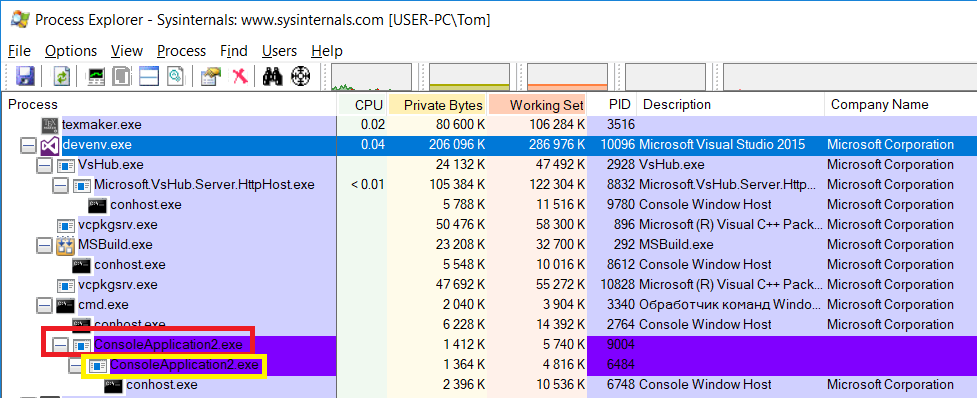
\includegraphics[width=\textwidth]{img/1}
  \caption{Структура процессов Visual Studio}
\end{figure}
На рисунке выделено два процесса \textbf{ConsoleApplication2.exe}, родительский с PID 9004, и дочерний, запущенный в контейнере с PID 6484.

Откроем каждый из процессов более подробно, и сравним их переменный окружения.
\begin{figure}[H]
  \centering
  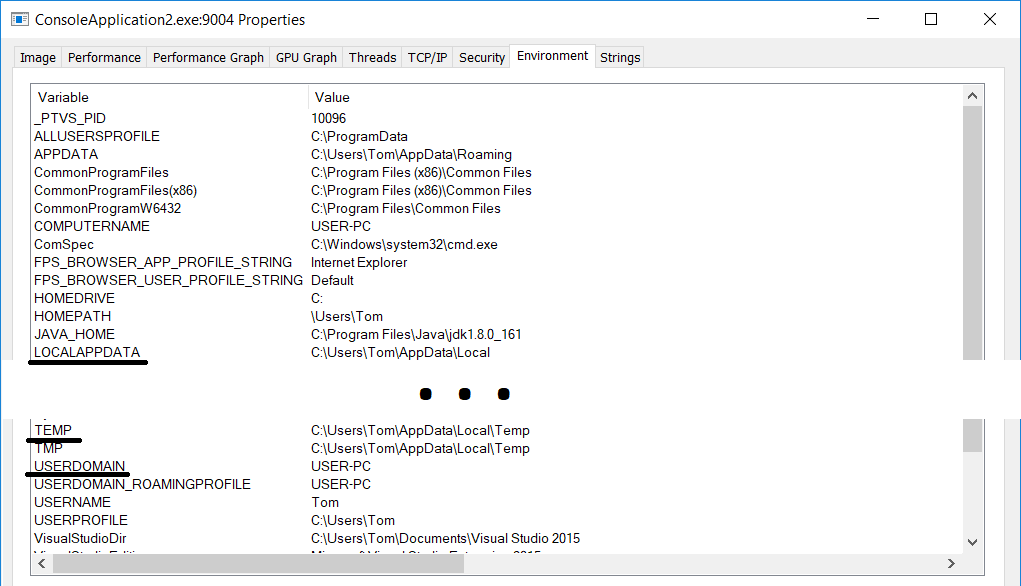
\includegraphics[width=\textwidth]{img/2}
  \caption{Переменные окружения родительского процесса}
\end{figure}
\begin{figure}[H]
  \centering
  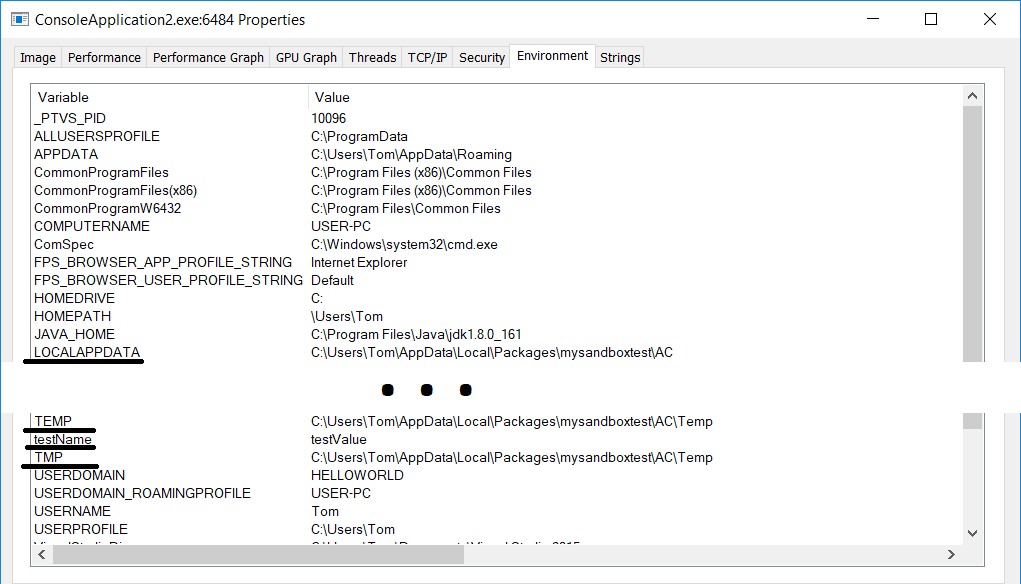
\includegraphics[width=\textwidth]{img/3}
  \caption{Переменные окружения процесса в контейнере}
\end{figure}
Как видно из рисунков:
\begin{enumerate}
\item Переменная с именем \textbf{testName} присутствует лишь в процессе запущенном в контейнере;
\item Значение переменной \textbf{USERDOMAIN} в контейнере является измененным;
\item Переменные \textbf{temp} и \textbf{localappdata} имеют иные пути, они были автоматически изменены без ручного изменния. Соответственно процесс в контейнере имеет доступ к этим папкам.
\begin{itemize}
\item Новый путь - C:\textbackslash Users\textbackslash Tom\textbackslash AppData\textbackslash Local\textbackslash Packages\textbackslash mysandboxtest\textbackslash AC\textbackslash Temp
\end{itemize}
\end{enumerate}


\subsection{Доступ к файлам}
Будет совершена проверка на доступ к:
\begin{enumerate}
\item Файлу находящимуся по пути
\begin{itemize}
\item C:\textbackslash Users\textbackslash Tom\textbackslash AppData\textbackslash Local\textbackslash Packages\textbackslash mysandboxtest \textbackslash AC\textbackslash Temp
\end{itemize} 
без предоставления каких-либо дополнительных разрешений;
\item Файлу на рабочем столе, к которому был дан доступ;
\item Файлу на рабочем столе, к которому не был дан доступ.
\end{enumerate}

\begin{lstlisting}[language={}, caption={Результат проверки}]
[+] Running filesystem test...
Opening of file C:\Users\Tom\AppData\Local\Packages\mysandboxtest\AC\Temp\allowed_test.txt was successful
Opening of file C:\Users\Tom\desktop\allowed_test.txt was successful
Opening of file C:\Users\Tom\desktop\blocked_test.txt returned access denied
\end{lstlisting}
Как видно из лога, доступ к файлу \textbf{blocked\_test.txt} был запрещен, а доступ к другим файлам был успешным, так как были выданы соответствующии права доступа.

\subsection{Доступ к сети}
Тестирование будет производиться путем открытия 80 порта, к следующим адреса:
\begin{itemize}
\item \textbf{108.177.14.138} (google.com);
\item \textbf{192.168.1.1} (локальный адрес роутера).
\end{itemize}
Тесты будут выполнены с использованием следующих: WELL\_KNOWN\_SID\_TYPE:
\begin{itemize}
\item WinCapabilityPrivateNetworkClientServerSid - доступ к локальной сети;
\item WinCapabilityInternetClientServerSid - доступ к сети "Интернет".
\end{itemize}
Без задачи каких-либо WELL\_KNOWN\_SID\_TYPE:
\begin{lstlisting}[language={}, caption={Полный запрет сети}]
Connection to 108.177.14.138 was blocked
Connection to 192.168.1.1 was blocked
\end{lstlisting}
WinCapabilityPrivateNetworkClientServerSid:
\begin{lstlisting}[language={}, caption={Доступ только к локальной сети}]
Connection to 108.177.14.138 was blocked
Connection to 192.168.1.1 was successful
\end{lstlisting}
WinCapabilityInternetClientServerSid:
\begin{lstlisting}[language={}, caption={Доступ только к сети "Интернет"}]
Connection to 108.177.14.138 was successful
Connection to 192.168.1.1 was blocked
\end{lstlisting}
Вместе:
\begin{lstlisting}[language={}, caption={Полный доступ к сети}]
Connection to 108.177.14.138 was successful
Connection to 192.168.1.1 was successful
\end{lstlisting}
Как видно из результатов, тестирование сети прошло успешно, доступ были предоставлены согласно выбранным WELL\_KNOWN\_SID\_TYPE.

\subsection{Список процессов}
Была написана функция \textbf{ProcessListTest} прикрепленная в приложении 5, суть которой заключается в выводе всех процессов в системе. Данная функция была запущена как из родительском процессе, так и в дочернем, изолированном процессе.

\begin{lstlisting}[language={}, caption={Список процессов из изолированного процесса}]
Found process: [System Process]
Found process: ConsoleApplication2.exe
Found process: conhost.exe
\end{lstlisting}
\begin{lstlisting}[language={}, caption={Список процессов из обычного процесса}]
Found process: [System Process]
Found process: System
Found process: smss.exe
Found process: csrss.exe
Found process: wininit.exe
Found process: services.exe
Found process: lsass.exe
Found process: svchost.exe
Found process: WUDFHost.exe
Found process: fontdrvhost.exe
Found process: svchost.exe
Found process: WUDFHost.exe
Found process: svchost.exe
...
\end{lstlisting}
Как видно из логов, изолированный процесс не видит прочих процессов в системе.


\section{Сравнение работы обычного и изолированного приложения}
Запустим все тесты сразу для обычного и изолированного процесса.

\begin{lstlisting}[language={}, caption={Лог обычного процесса}]
[+] Running filesystem test...
Path of %temp%: C:\Users\Tom\AppData\Local\Temp
Path of %localappdata%: C:\Users\Tom\AppData\Local
Opening of file C:\Users\Tom\AppData\Local\Temp\allowed_test.txt was successful
Opening of file C:\Users\Tom\desktop\allowed_test.txt was successful
Opening of file C:\Users\Tom\desktop\blocked_test.txt was successful
[+] Filesystem testing done

[+] Running network test...
Connection to 108.177.14.138 was successful
Connection to 192.168.1.1 was successful
[+] Network testing done

[+] Running process list testing...
Found process: [System Process]
Found process: System
Found process: smss.exe
Found process: csrss.exe
Found process: wininit.exe
Found process: csrss.exe
Found process: services.exe
...
Found process: svchost.exe
Found process: cmd.exe
Found process: conhost.exe
Found process: ConsoleApplication2.exe
[+] Process list testing done
\end{lstlisting}
\begin{lstlisting}[language={}, caption={Лог изолированного процесса}]
[+] Running filesystem test...
Path of %temp%: C:\Users\Tom\AppData\Local\Packages\mysandboxtest\AC\Temp
Path of %localappdata%: C:\Users\Tom\AppData\Local\Packages\mysandboxtest\AC
Opening of file C:\Users\Tom\AppData\Local\Packages\mysandboxtest\AC\Temp\allowed_test.txt was successful
Opening of file C:\Users\Tom\desktop\allowed_test.txt was successful
Opening of file C:\Users\Tom\desktop\blocked_test.txt returned access denied
[+] Filesystem testing done

[+] Running network test...
Connection to 108.177.14.138 was blocked
Connection to 192.168.1.1 was blocked
[+] Network testing done

[+] Running process list testing...
Found process: [System Process]
Found process: ConsoleApplication2.exe
Found process: conhost.exe
[+] Process list testing done
\end{lstlisting}
Как видно из логов, для обычного процесса доступ к сети был полностью разрешен, а в изолированном полностью заблокирован. Тоже касается файлов, обычный процесс смог получить доступ ко всем файлам, а изолированный лишь к доступным.

Рассмотрим работу прочих приложений.

Запуск блокнота по пути - C:\textbackslash Windows\textbackslash notepad.exe происходит без каких-либо проблем, что говорит о возможности подгрузки GUI.
Из изолированного блокнота был сохранен файл по пути
\begin{center}
C:\textbackslash Users\textbackslash Tom\textbackslash AppData\textbackslash Local\textbackslash Packages\textbackslash mysandboxtest \textbackslash AC\textbackslash Temp
\end{center}
А из не изолированного по пути \textbf{E:\textbackslash}. Далее было произведено сравнение свойств файлов.
\begin{figure}[H]
  \centering
  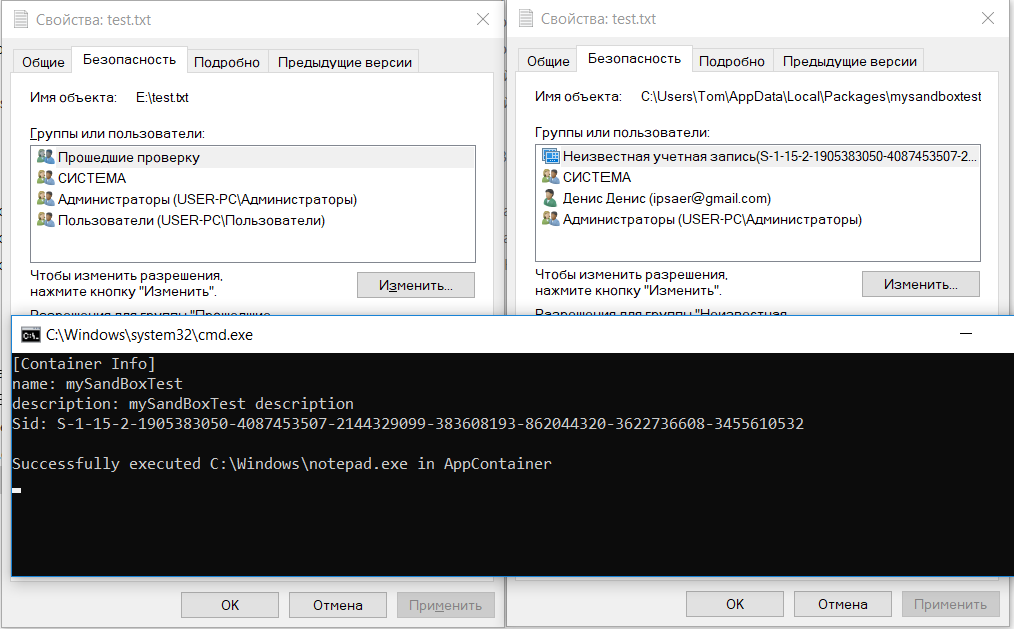
\includegraphics[width=\textwidth]{img/10}
  \caption{Сравнение свойств файлов}
\end{figure}
Как видно из рисунка, на вкладке безопасность, у файла справа первой строкой записано - \textbf{Неизвестная учетная запись(S-15-2-19...)}. И если взглянуть на вывод консоли, становиться понятно что неизветная учетная запись является SID контейнера. То есть в данном случае вместо привычного пользователя или группы выступает идентификатор контейнера.\\\\
Запуск более масштабных приложений: Google Chrome, Internet Explorer и т.д. не приводил к успешному запуску. Процесс данный программ был создан, но никаких ошибок или окон GUI не последовало.

Это скорее всего связано с тем, что у программ имеются зависимости от прочих сервисов, настроек реестра, прочих файлов(то что проиходит во время установки программы)



\clearpage
\addcontentsline{toc}{section}{Заключение}
\section*{Заключение}
В данной работе была рассмотрена изоляция процессов в Windows средствами LPAC. Технология Application Container и LPAC являются сравнительно новыми(2017 год). Во время чтения используемых функций на msdn было видно что некоторые параметры еще не используется в полной мере или вовсе пока являются заглушками.

Если сравнивать с Linux решениями по контейнерезации, то пока использование Application Container несколько затруднено из-за:
\begin{itemize}
\item Отсутствует какой-либо репозиторий с готовыми контейнерами;
\item Средство пока еще слабо документировано.
\end{itemize}
Но данные проблемы решаемы, и уже сейчас идет создание открытого репозитория с контейнерами.

В работе была продемонстрирована работы с ФС, сетевыми функциями, переменными окружения, процессами системы из изолированного процесса. Все возможности изолированного процесса как и ожидлось были жестко ограничены, без расширения соответствующих прав доступа.

В работе были произведены попытки запуска более масштабных приложений, наподобии браузеров, но это не увенчалось успехом. Это связано с тем, что первоначальная цель контейнеризации была именно изоляция процессов, что сейчас широко применяется в микросервисах.

Помимо микросервисов, технология контейнеризации широко применяется в антивирусных программах. В которых необходимо оградить внутренние процесс от внеших вмешательств. С приходом технологии Application Container на ОС семейства Windows появляется возможность изолировать процессы используя нативные возможности системы.

%------------------------------------------------------------------------------

\clearpage
\addcontentsline{toc}{section}{Список использованных источников}
\bibliography{thesis}
\bibliographystyle{ugost2008}

\nocite{windowscontainers}
\nocite{jail}
\nocite{Docker}


\clearpage
\addcontentsline{toc}{section}{Приложения}
\subsection*{Приложение 1. Main.cpp} \label{p1:1}
\addcontentsline{toc}{subsection}{Приложение 1. main.cpp}
\textbf{Точка входа в программу}
\lstinputlisting[caption=Main.cpp]{code/Main.cpp}
\subsection*{Приложение 2. ContainerCreate.h} \label{p1:1}
\addcontentsline{toc}{subsection}{Приложение 2. ContainerCreate.h}
\textbf{Заголовочный файл ContainerCreate.h}
\lstinputlisting[caption=ContainerCreate.h]{code/ContainerCreate.h}
\subsection*{Приложение 3. ContainerCreate.cpp} \label{p1:1}
\addcontentsline{toc}{subsection}{Приложение 3. ContainerCreate.cpp}
\textbf{Файл по запуску контейнера, настройке и запуску приложения}
\lstinputlisting[caption=ContainerCreate.cpp]{code/ContainerCreate.cpp}
\subsection*{Приложение 4. ContainerTest.h} \label{p1:1}
\addcontentsline{toc}{subsection}{Приложение 4. ContainerTest.h}
\textbf{Заголовочный файл ContainerTest.h}
\lstinputlisting[caption=ContainerTest.h]{code/ContainerTest.h}
\subsection*{Приложение 5. ContainerTest.cpp} \label{p1:1}
\addcontentsline{toc}{subsection}{Приложение 5. ContainerTest.cpp}
\textbf{Файл с тестами для изолированного процесса}
\lstinputlisting[caption=ContainerTest.cpp]{code/ContainerTest.cpp}
\subsection*{Приложение 6. Структура проекта} \label{p1:1}
\addcontentsline{toc}{subsection}{Приложение 6. Структура проекта}
Проект состоит из:
\begin{itemize}
\item 2 заголовочных файлов:
\begin{itemize}
\item ContainerCreate.h;
\item ContainerTest.h.
\end{itemize}
\item 3 файлов с исходным кодом:
\begin{itemize}
\item Main.cpp;
\item ContainerCreate.cpp;
\item ContainerTest.cpp.
\end{itemize}
\end{itemize}


\end{document}
